% Options for packages loaded elsewhere
\PassOptionsToPackage{unicode}{hyperref}
\PassOptionsToPackage{hyphens}{url}
\PassOptionsToPackage{dvipsnames,svgnames,x11names}{xcolor}
%
\documentclass[
  letterpaper,
  DIV=11,
  numbers=noendperiod]{scrartcl}

\usepackage{amsmath,amssymb}
\usepackage{iftex}
\ifPDFTeX
  \usepackage[T1]{fontenc}
  \usepackage[utf8]{inputenc}
  \usepackage{textcomp} % provide euro and other symbols
\else % if luatex or xetex
  \usepackage{unicode-math}
  \defaultfontfeatures{Scale=MatchLowercase}
  \defaultfontfeatures[\rmfamily]{Ligatures=TeX,Scale=1}
\fi
\usepackage{lmodern}
\ifPDFTeX\else  
    % xetex/luatex font selection
\fi
% Use upquote if available, for straight quotes in verbatim environments
\IfFileExists{upquote.sty}{\usepackage{upquote}}{}
\IfFileExists{microtype.sty}{% use microtype if available
  \usepackage[]{microtype}
  \UseMicrotypeSet[protrusion]{basicmath} % disable protrusion for tt fonts
}{}
\makeatletter
\@ifundefined{KOMAClassName}{% if non-KOMA class
  \IfFileExists{parskip.sty}{%
    \usepackage{parskip}
  }{% else
    \setlength{\parindent}{0pt}
    \setlength{\parskip}{6pt plus 2pt minus 1pt}}
}{% if KOMA class
  \KOMAoptions{parskip=half}}
\makeatother
\usepackage{xcolor}
\setlength{\emergencystretch}{3em} % prevent overfull lines
\setcounter{secnumdepth}{5}
% Make \paragraph and \subparagraph free-standing
\makeatletter
\ifx\paragraph\undefined\else
  \let\oldparagraph\paragraph
  \renewcommand{\paragraph}{
    \@ifstar
      \xxxParagraphStar
      \xxxParagraphNoStar
  }
  \newcommand{\xxxParagraphStar}[1]{\oldparagraph*{#1}\mbox{}}
  \newcommand{\xxxParagraphNoStar}[1]{\oldparagraph{#1}\mbox{}}
\fi
\ifx\subparagraph\undefined\else
  \let\oldsubparagraph\subparagraph
  \renewcommand{\subparagraph}{
    \@ifstar
      \xxxSubParagraphStar
      \xxxSubParagraphNoStar
  }
  \newcommand{\xxxSubParagraphStar}[1]{\oldsubparagraph*{#1}\mbox{}}
  \newcommand{\xxxSubParagraphNoStar}[1]{\oldsubparagraph{#1}\mbox{}}
\fi
\makeatother

\usepackage{color}
\usepackage{fancyvrb}
\newcommand{\VerbBar}{|}
\newcommand{\VERB}{\Verb[commandchars=\\\{\}]}
\DefineVerbatimEnvironment{Highlighting}{Verbatim}{commandchars=\\\{\}}
% Add ',fontsize=\small' for more characters per line
\usepackage{framed}
\definecolor{shadecolor}{RGB}{241,243,245}
\newenvironment{Shaded}{\begin{snugshade}}{\end{snugshade}}
\newcommand{\AlertTok}[1]{\textcolor[rgb]{0.68,0.00,0.00}{#1}}
\newcommand{\AnnotationTok}[1]{\textcolor[rgb]{0.37,0.37,0.37}{#1}}
\newcommand{\AttributeTok}[1]{\textcolor[rgb]{0.40,0.45,0.13}{#1}}
\newcommand{\BaseNTok}[1]{\textcolor[rgb]{0.68,0.00,0.00}{#1}}
\newcommand{\BuiltInTok}[1]{\textcolor[rgb]{0.00,0.23,0.31}{#1}}
\newcommand{\CharTok}[1]{\textcolor[rgb]{0.13,0.47,0.30}{#1}}
\newcommand{\CommentTok}[1]{\textcolor[rgb]{0.37,0.37,0.37}{#1}}
\newcommand{\CommentVarTok}[1]{\textcolor[rgb]{0.37,0.37,0.37}{\textit{#1}}}
\newcommand{\ConstantTok}[1]{\textcolor[rgb]{0.56,0.35,0.01}{#1}}
\newcommand{\ControlFlowTok}[1]{\textcolor[rgb]{0.00,0.23,0.31}{\textbf{#1}}}
\newcommand{\DataTypeTok}[1]{\textcolor[rgb]{0.68,0.00,0.00}{#1}}
\newcommand{\DecValTok}[1]{\textcolor[rgb]{0.68,0.00,0.00}{#1}}
\newcommand{\DocumentationTok}[1]{\textcolor[rgb]{0.37,0.37,0.37}{\textit{#1}}}
\newcommand{\ErrorTok}[1]{\textcolor[rgb]{0.68,0.00,0.00}{#1}}
\newcommand{\ExtensionTok}[1]{\textcolor[rgb]{0.00,0.23,0.31}{#1}}
\newcommand{\FloatTok}[1]{\textcolor[rgb]{0.68,0.00,0.00}{#1}}
\newcommand{\FunctionTok}[1]{\textcolor[rgb]{0.28,0.35,0.67}{#1}}
\newcommand{\ImportTok}[1]{\textcolor[rgb]{0.00,0.46,0.62}{#1}}
\newcommand{\InformationTok}[1]{\textcolor[rgb]{0.37,0.37,0.37}{#1}}
\newcommand{\KeywordTok}[1]{\textcolor[rgb]{0.00,0.23,0.31}{\textbf{#1}}}
\newcommand{\NormalTok}[1]{\textcolor[rgb]{0.00,0.23,0.31}{#1}}
\newcommand{\OperatorTok}[1]{\textcolor[rgb]{0.37,0.37,0.37}{#1}}
\newcommand{\OtherTok}[1]{\textcolor[rgb]{0.00,0.23,0.31}{#1}}
\newcommand{\PreprocessorTok}[1]{\textcolor[rgb]{0.68,0.00,0.00}{#1}}
\newcommand{\RegionMarkerTok}[1]{\textcolor[rgb]{0.00,0.23,0.31}{#1}}
\newcommand{\SpecialCharTok}[1]{\textcolor[rgb]{0.37,0.37,0.37}{#1}}
\newcommand{\SpecialStringTok}[1]{\textcolor[rgb]{0.13,0.47,0.30}{#1}}
\newcommand{\StringTok}[1]{\textcolor[rgb]{0.13,0.47,0.30}{#1}}
\newcommand{\VariableTok}[1]{\textcolor[rgb]{0.07,0.07,0.07}{#1}}
\newcommand{\VerbatimStringTok}[1]{\textcolor[rgb]{0.13,0.47,0.30}{#1}}
\newcommand{\WarningTok}[1]{\textcolor[rgb]{0.37,0.37,0.37}{\textit{#1}}}

\providecommand{\tightlist}{%
  \setlength{\itemsep}{0pt}\setlength{\parskip}{0pt}}\usepackage{longtable,booktabs,array}
\usepackage{calc} % for calculating minipage widths
% Correct order of tables after \paragraph or \subparagraph
\usepackage{etoolbox}
\makeatletter
\patchcmd\longtable{\par}{\if@noskipsec\mbox{}\fi\par}{}{}
\makeatother
% Allow footnotes in longtable head/foot
\IfFileExists{footnotehyper.sty}{\usepackage{footnotehyper}}{\usepackage{footnote}}
\makesavenoteenv{longtable}
\usepackage{graphicx}
\makeatletter
\def\maxwidth{\ifdim\Gin@nat@width>\linewidth\linewidth\else\Gin@nat@width\fi}
\def\maxheight{\ifdim\Gin@nat@height>\textheight\textheight\else\Gin@nat@height\fi}
\makeatother
% Scale images if necessary, so that they will not overflow the page
% margins by default, and it is still possible to overwrite the defaults
% using explicit options in \includegraphics[width, height, ...]{}
\setkeys{Gin}{width=\maxwidth,height=\maxheight,keepaspectratio}
% Set default figure placement to htbp
\makeatletter
\def\fps@figure{htbp}
\makeatother
% definitions for citeproc citations
\NewDocumentCommand\citeproctext{}{}
\NewDocumentCommand\citeproc{mm}{%
  \begingroup\def\citeproctext{#2}\cite{#1}\endgroup}
\makeatletter
 % allow citations to break across lines
 \let\@cite@ofmt\@firstofone
 % avoid brackets around text for \cite:
 \def\@biblabel#1{}
 \def\@cite#1#2{{#1\if@tempswa , #2\fi}}
\makeatother
\newlength{\cslhangindent}
\setlength{\cslhangindent}{1.5em}
\newlength{\csllabelwidth}
\setlength{\csllabelwidth}{3em}
\newenvironment{CSLReferences}[2] % #1 hanging-indent, #2 entry-spacing
 {\begin{list}{}{%
  \setlength{\itemindent}{0pt}
  \setlength{\leftmargin}{0pt}
  \setlength{\parsep}{0pt}
  % turn on hanging indent if param 1 is 1
  \ifodd #1
   \setlength{\leftmargin}{\cslhangindent}
   \setlength{\itemindent}{-1\cslhangindent}
  \fi
  % set entry spacing
  \setlength{\itemsep}{#2\baselineskip}}}
 {\end{list}}
\usepackage{calc}
\newcommand{\CSLBlock}[1]{\hfill\break\parbox[t]{\linewidth}{\strut\ignorespaces#1\strut}}
\newcommand{\CSLLeftMargin}[1]{\parbox[t]{\csllabelwidth}{\strut#1\strut}}
\newcommand{\CSLRightInline}[1]{\parbox[t]{\linewidth - \csllabelwidth}{\strut#1\strut}}
\newcommand{\CSLIndent}[1]{\hspace{\cslhangindent}#1}

\KOMAoption{captions}{tableheading}
\makeatletter
\@ifpackageloaded{caption}{}{\usepackage{caption}}
\AtBeginDocument{%
\ifdefined\contentsname
  \renewcommand*\contentsname{Table of contents}
\else
  \newcommand\contentsname{Table of contents}
\fi
\ifdefined\listfigurename
  \renewcommand*\listfigurename{List of Figures}
\else
  \newcommand\listfigurename{List of Figures}
\fi
\ifdefined\listtablename
  \renewcommand*\listtablename{List of Tables}
\else
  \newcommand\listtablename{List of Tables}
\fi
\ifdefined\figurename
  \renewcommand*\figurename{Figure}
\else
  \newcommand\figurename{Figure}
\fi
\ifdefined\tablename
  \renewcommand*\tablename{Table}
\else
  \newcommand\tablename{Table}
\fi
}
\@ifpackageloaded{float}{}{\usepackage{float}}
\floatstyle{ruled}
\@ifundefined{c@chapter}{\newfloat{codelisting}{h}{lop}}{\newfloat{codelisting}{h}{lop}[chapter]}
\floatname{codelisting}{Listing}
\newcommand*\listoflistings{\listof{codelisting}{List of Listings}}
\makeatother
\makeatletter
\makeatother
\makeatletter
\@ifpackageloaded{caption}{}{\usepackage{caption}}
\@ifpackageloaded{subcaption}{}{\usepackage{subcaption}}
\makeatother

\ifLuaTeX
  \usepackage{selnolig}  % disable illegal ligatures
\fi
\usepackage{bookmark}

\IfFileExists{xurl.sty}{\usepackage{xurl}}{} % add URL line breaks if available
\urlstyle{same} % disable monospaced font for URLs
\hypersetup{
  pdftitle={My title},
  pdfauthor={First author; Yongqi Liu; Yuxuan Wei},
  colorlinks=true,
  linkcolor={blue},
  filecolor={Maroon},
  citecolor={Blue},
  urlcolor={Blue},
  pdfcreator={LaTeX via pandoc}}


\title{My title\thanks{Code and data are available at:
{[}https://github.com/wyx827/2024USpresidentialelection.git{]}.}}
\usepackage{etoolbox}
\makeatletter
\providecommand{\subtitle}[1]{% add subtitle to \maketitle
  \apptocmd{\@title}{\par {\large #1 \par}}{}{}
}
\makeatother
\subtitle{My subtitle if needed}
\author{First author \and Yongqi Liu \and Yuxuan Wei}
\date{October 23, 2024}

\begin{document}
\maketitle
\begin{abstract}
First sentence. Second sentence. Third sentence. Fourth sentence.
\end{abstract}


\begin{Shaded}
\begin{Highlighting}[]
\CommentTok{\#install.packages("tidymodels")}
\FunctionTok{library}\NormalTok{(tidyverse)}
\end{Highlighting}
\end{Shaded}

\begin{verbatim}
-- Attaching core tidyverse packages ------------------------ tidyverse 2.0.0 --
v dplyr     1.1.4     v readr     2.1.5
v forcats   1.0.0     v stringr   1.5.1
v ggplot2   3.5.1     v tibble    3.2.1
v lubridate 1.9.3     v tidyr     1.3.1
v purrr     1.0.2     
-- Conflicts ------------------------------------------ tidyverse_conflicts() --
x dplyr::filter() masks stats::filter()
x dplyr::lag()    masks stats::lag()
i Use the conflicted package (<http://conflicted.r-lib.org/>) to force all conflicts to become errors
\end{verbatim}

\begin{Shaded}
\begin{Highlighting}[]
\FunctionTok{library}\NormalTok{(ggplot2)}
\NormalTok{analysis\_data }\OtherTok{\textless{}{-}} \FunctionTok{read\_csv}\NormalTok{(here}\SpecialCharTok{::}\FunctionTok{here}\NormalTok{(}\StringTok{"data/02{-}analysis\_data/cleaned\_US\_voting.csv"}\NormalTok{))}
\end{Highlighting}
\end{Shaded}

\begin{verbatim}
Rows: 1683 Columns: 11
-- Column specification --------------------------------------------------------
Delimiter: ","
chr  (5): pollster_rating_name, methodology, state, candidate_name, populati...
dbl  (4): numeric_grade, sample_size, percent, transparency_score
date (2): start_date, end_date

i Use `spec()` to retrieve the full column specification for this data.
i Specify the column types or set `show_col_types = FALSE` to quiet this message.
\end{verbatim}

\section{Introduction}\label{introduction}

Overview paragraph

Estimand paragraph

Results paragraph

Why it matters paragraph

Telegraphing paragraph: The remainder of this paper is structured as
follows. Section~\ref{sec-data}\ldots.

\section{Data}\label{sec-data}

\subsection{Overview}\label{overview}

We use the statistical programming language R (R Core Team 2023)\ldots.
Following Alexander (2023), we consider\ldots{}

Overview text

\subsection{Measurement}\label{measurement}

Some paragraphs about how we go from a phenomena in the world to an
entry in the dataset.

\subsection{Outcome variables}\label{outcome-variables}

Add graphs, tables and text. Use sub-sub-headings for each outcome
variable or update the subheading to be singular.

Some of our data is of penguins (\textbf{?@fig-bills}),

Talk more about it.

And also planes (\textbf{?@fig-planes}). (You can change the height and
width, but don't worry about doing that until you have finished every
other aspect of the paper - Quarto will try to make it look nice and the
defaults usually work well once you have enough text.)

Talk way more about it.

\subsection{Predictor variables}\label{predictor-variables}

Add graphs, tables and text.

Use sub-sub-headings for each outcome variable and feel free to combine
a few into one if they go together naturally.

\section{Model}\label{model}

To model Donald Trump's polling percentages over time, we employed a
Bayesian linear regression framework. Bayesian methods provide a
flexible approach to inference by incorporating prior beliefs and
updating them with observed data, allowing us to quantify uncertainty in
both parameter estimates and predictions.

Here we briefly describe the Bayesian model used to investigate the
winning probability of Trump. Background details and diagnostics are
included in Appendix~\ref{sec-model-details}.

\subsection{Multiple Linear Regression Model
Overview}\label{multiple-linear-regression-model-overview}

The model now predicts Trump's polling percentage (percent) using the
following predictors:

\begin{itemize}
\tightlist
\item
  Numeric Grade (numeric\_grade): Reflects the quality rating of the
  pollster.
\item
  Sample Size (sample\_size): The number of respondents in the poll.
\item
  State (state): A categorical variable for different U.S. states.
\item
  Transparency Score (transparency\_score): A measure of how transparent
  the polling data and methodology are.
\item
  End Date (end\_date): The date the poll was completed, which might
  capture trends over time.
\end{itemize}

The model takes the form: The model takes the form:

\section{\#Interpretation of
Coefficients:}\label{interpretation-of-coefficients}

\begin{itemize}
\tightlist
\item
  Intercept (\beta\_0): This is the predicted Trump polling percentage
  when all predictors (numeric grade, sample size, state, transparency
  score, and end date) are at their baseline or zero value.
\item
  Numeric Grade (\beta\_1): This coefficient measures how much Trump's
  polling percentage changes as the pollster's numeric grade increases.
  A positive and significant coefficient would indicate that
  higher-rated pollsters report better polling numbers for Trump, while
  a negative coefficient would suggest the opposite.
\item
  Sample Size (\beta\_2): This measures the impact of the number of
  respondents on Trump's polling percentage. A positive coefficient
  would indicate that larger sample sizes are associated with higher
  polling percentages for Trump.
\item
  State (\beta\_3): The coefficients for the state variable represent
  differences in Trump's polling percentage in each state compared to
  the reference state (baseline category). For example, if the
  coefficient for Florida is negative, it means Trump polls lower in
  Florida compared to the reference state.
\item
  Transparency Score (\beta\_4): This coefficient shows how much Trump's
  polling percentage is affected by the transparency of the poll. A
  positive coefficient would indicate that polls with higher
  transparency tend to report higher polling percentages for Trump,
  whereas a negative coefficient would imply the opposite.
\item
  End Date (\beta\_5): The end date is a time-related variable,
  capturing trends over time. A positive and significant coefficient
  would suggest that Trump's polling percentage has increased as the
  election date approaches, while a negative coefficient would suggest a
  decrease in his polling numbers over time.
\end{itemize}

\subsection{Interpretation}\label{interpretation}

The posterior distributions of the parameters allow us to quantify the
uncertainty around each effect: - The coefficient for end\_date informs
us about how Trump's polling percentages have evolved over time. A
positive coefficient would suggest an upward trend, while a negative
coefficient would indicate a decline. - The coefficient for
numeric\_grade captures the impact of pollster quality on the polling
percentage. High-quality pollsters may produce different estimates
compared to lower-quality ones. - The state-level effects account for
regional differences in Trump's support. Some states may show
significantly higher or lower levels of support, even after adjusting
for the time of the poll and pollster quality.

\section{Model Evalutation}\label{model-evalutation}

\begin{itemize}
\tightlist
\item
  R-squared Table~\ref{tbl-summary} shows the summary table for the
  model. And then evaluate it on the test set. It appears as though the
  model is having difficulty identifying Trump supporters.
\end{itemize}

\begin{longtable}[]{@{}
  >{\raggedright\arraybackslash}p{(\columnwidth - 8\tabcolsep) * \real{0.2985}}
  >{\raggedleft\arraybackslash}p{(\columnwidth - 8\tabcolsep) * \real{0.1343}}
  >{\raggedleft\arraybackslash}p{(\columnwidth - 8\tabcolsep) * \real{0.1642}}
  >{\raggedleft\arraybackslash}p{(\columnwidth - 8\tabcolsep) * \real{0.1194}}
  >{\raggedleft\arraybackslash}p{(\columnwidth - 8\tabcolsep) * \real{0.2836}}@{}}

\caption{\label{tbl-summary}Relationship between wing length and width}

\tabularnewline

\caption{Regression Model Coefficients}\tabularnewline
\toprule\noalign{}
\begin{minipage}[b]{\linewidth}\raggedright
\end{minipage} & \begin{minipage}[b]{\linewidth}\raggedleft
Estimate
\end{minipage} & \begin{minipage}[b]{\linewidth}\raggedleft
Std. Error
\end{minipage} & \begin{minipage}[b]{\linewidth}\raggedleft
t value
\end{minipage} & \begin{minipage}[b]{\linewidth}\raggedleft
Pr(\textgreater\textbar t\textbar)
\end{minipage} \\
\midrule\noalign{}
\endfirsthead
\toprule\noalign{}
\begin{minipage}[b]{\linewidth}\raggedright
\end{minipage} & \begin{minipage}[b]{\linewidth}\raggedleft
Estimate
\end{minipage} & \begin{minipage}[b]{\linewidth}\raggedleft
Std. Error
\end{minipage} & \begin{minipage}[b]{\linewidth}\raggedleft
t value
\end{minipage} & \begin{minipage}[b]{\linewidth}\raggedleft
Pr(\textgreater\textbar t\textbar)
\end{minipage} \\
\midrule\noalign{}
\endhead
\bottomrule\noalign{}
\endlastfoot
(Intercept) & -67.184 & 14.445 & -4.651 & 0.000 \\
numeric\_grade & 0.914 & 1.006 & 0.909 & 0.364 \\
sample\_size & 0.000 & 0.000 & 0.205 & 0.838 \\
stateArizona & -5.020 & 2.582 & -1.944 & 0.052 \\
stateArkansas & 5.569 & 4.380 & 1.272 & 0.204 \\
stateCalifornia & -18.345 & 2.738 & -6.699 & 0.000 \\
stateColorado & -13.340 & 3.002 & -4.443 & 0.000 \\
stateConnecticut & -13.480 & 3.574 & -3.772 & 0.000 \\
stateFlorida & -3.214 & 2.740 & -1.173 & 0.241 \\
stateGeorgia & -4.814 & 2.573 & -1.871 & 0.062 \\
stateIdaho & 3.467 & 4.379 & 0.792 & 0.429 \\
stateIllinois & -14.064 & 3.275 & -4.294 & 0.000 \\
stateIndiana & 0.902 & 3.268 & 0.276 & 0.783 \\
stateIowa & -4.692 & 3.101 & -1.513 & 0.131 \\
stateKansas & -0.798 & 3.275 & -0.244 & 0.808 \\
stateMaine & -10.182 & 2.726 & -3.735 & 0.000 \\
stateMaryland & -20.244 & 2.998 & -6.753 & 0.000 \\
stateMassachusetts & -22.543 & 2.753 & -8.190 & 0.000 \\
stateMichigan & -6.635 & 2.576 & -2.576 & 0.010 \\
stateMinnesota & -10.250 & 2.684 & -3.819 & 0.000 \\
stateMissouri & 1.087 & 2.803 & 0.388 & 0.698 \\
stateMontana & 1.379 & 2.784 & 0.495 & 0.620 \\
stateNational & -7.935 & 2.546 & -3.117 & 0.002 \\
stateNebraska & -7.528 & 2.782 & -2.706 & 0.007 \\
stateNevada & -5.617 & 2.594 & -2.165 & 0.031 \\
stateNew Hampshire & -8.778 & 2.655 & -3.306 & 0.001 \\
stateNew Jersey & -15.189 & 3.577 & -4.246 & 0.000 \\
stateNew Mexico & -10.980 & 3.099 & -3.543 & 0.000 \\
stateNew York & -15.239 & 2.633 & -5.789 & 0.000 \\
stateNorth Carolina & -4.783 & 2.582 & -1.853 & 0.064 \\
stateNorth Dakota & 2.970 & 4.380 & 0.678 & 0.498 \\
stateOhio & -2.796 & 2.677 & -1.045 & 0.296 \\
stateOklahoma & 8.450 & 4.385 & 1.927 & 0.054 \\
stateOregon & -14.974 & 4.385 & -3.415 & 0.001 \\
statePennsylvania & -6.375 & 2.568 & -2.483 & 0.013 \\
stateRhode Island & -13.374 & 2.994 & -4.467 & 0.000 \\
stateSouth Carolina & -1.939 & 4.376 & -0.443 & 0.658 \\
stateSouth Dakota & 0.394 & 3.096 & 0.127 & 0.899 \\
stateTennessee & 3.624 & 4.378 & 0.828 & 0.408 \\
stateTexas & -3.825 & 2.681 & -1.427 & 0.154 \\
stateUtah & -3.243 & 4.385 & -0.740 & 0.460 \\
stateVermont & -23.452 & 3.581 & -6.549 & 0.000 \\
stateVirginia & -9.518 & 2.663 & -3.575 & 0.000 \\
stateWashington & -15.876 & 3.264 & -4.864 & 0.000 \\
stateWest Virginia & 8.265 & 4.379 & 1.887 & 0.059 \\
stateWisconsin & -6.444 & 2.571 & -2.506 & 0.012 \\
stateWyoming & 15.921 & 4.377 & 3.637 & 0.000 \\
transparency\_score & -0.646 & 0.088 & -7.383 & 0.000 \\
end\_date & 0.006 & 0.001 & 8.880 & 0.000 \\

\end{longtable}

\section{Diagnostic plots for the
model}\label{diagnostic-plots-for-the-model}

\begin{figure}

\centering{

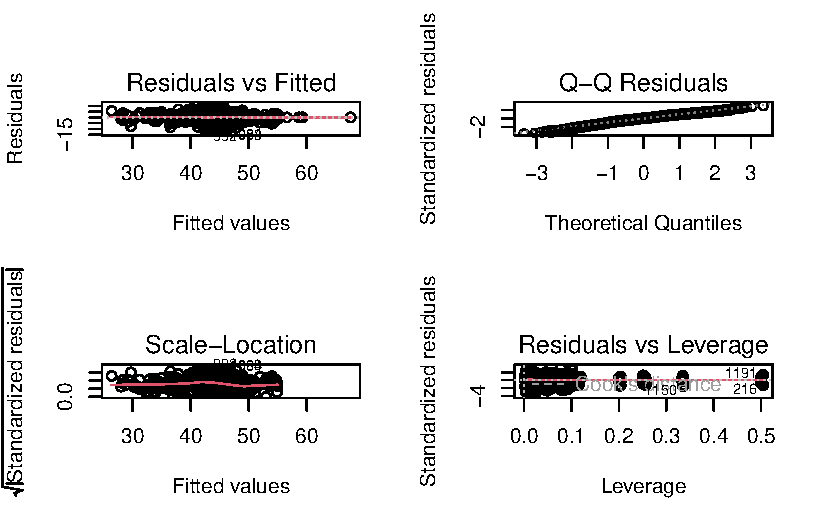
\includegraphics{paper_files/figure-pdf/fig-diagnosis-1.pdf}

}

\caption{\label{fig-diagnosis}}

\end{figure}%

\begin{Shaded}
\begin{Highlighting}[]
\FunctionTok{library}\NormalTok{(car)}
\end{Highlighting}
\end{Shaded}

\begin{verbatim}
Loading required package: carData
\end{verbatim}

\begin{verbatim}

Attaching package: 'car'
\end{verbatim}

\begin{verbatim}
The following object is masked from 'package:dplyr':

    recode
\end{verbatim}

\begin{verbatim}
The following object is masked from 'package:purrr':

    some
\end{verbatim}

\begin{Shaded}
\begin{Highlighting}[]
\FunctionTok{vif}\NormalTok{(regression\_model)}
\end{Highlighting}
\end{Shaded}

\begin{verbatim}
                       GVIF Df GVIF^(1/(2*Df))
numeric_grade      1.294110  1        1.137590
sample_size        1.289750  1        1.135672
state              2.082151 44        1.008369
transparency_score 1.263558  1        1.124081
end_date           1.309491  1        1.144330
\end{verbatim}

\subsubsection{Model justification}\label{model-justification}

We expect a positive relationship between the size of the wings and time
spent aloft. In particular\ldots{}

We can use maths by including latex between dollar signs, for instance
\(\theta\).

\section{Results}\label{results}

\subsection{Predict and Combine with Electroal College to
Predict}\label{predict-and-combine-with-electroal-college-to-predict}

\begin{longtable}[]{@{}lrrl@{}}

\caption{\label{tbl-prediction}Prediction for Trump}

\tabularnewline

\caption{Prediction for Trump by State}\tabularnewline
\toprule\noalign{}
State & Trump Predicted \% & Electoral Votes & Winner \\
\midrule\noalign{}
\endfirsthead
\toprule\noalign{}
State & Trump Predicted \% & Electoral Votes & Winner \\
\midrule\noalign{}
\endhead
\bottomrule\noalign{}
\endlastfoot
Alaska & 53.00 & 3 & Trump \\
Arizona & 47.62 & 11 & Harris \\
Arkansas & 56.60 & 6 & Trump \\
California & 34.39 & 55 & Harris \\
Colorado & 37.60 & 9 & Harris \\
Connecticut & 39.09 & 7 & Harris \\
Florida & 48.89 & 29 & Harris \\
Georgia & 47.71 & 16 & Harris \\
Idaho & 54.50 & 4 & Trump \\
Illinois & 36.37 & 20 & Harris \\
Indiana & 53.73 & 11 & Trump \\
Iowa & 46.68 & 6 & Harris \\
Kansas & 49.63 & 6 & Harris \\
Maine & 41.13 & 2 & Harris \\
Maryland & 32.88 & 10 & Harris \\
Massachusetts & 29.80 & 11 & Harris \\
Michigan & 45.92 & 15 & Harris \\
Minnesota & 42.40 & 10 & Harris \\
Missouri & 52.51 & 10 & Trump \\
Montana & 54.20 & 3 & Trump \\
Nebraska & 45.16 & 5 & Harris \\
Nevada & 47.00 & 6 & Harris \\
New Hampshire & 42.86 & 4 & Harris \\
New Jersey & 37.60 & 14 & Harris \\
New Mexico & 42.05 & 5 & Harris \\
New York & 37.45 & 29 & Harris \\
North Carolina & 47.98 & 16 & Harris \\
North Dakota & 54.00 & 3 & Trump \\
Ohio & 49.58 & 18 & Harris \\
Oklahoma & 58.70 & 7 & Trump \\
Oregon & 35.30 & 6 & Harris \\
Pennsylvania & 46.28 & 20 & Harris \\
Rhode Island & 39.12 & 4 & Harris \\
South Carolina & 50.60 & 9 & Trump \\
South Dakota & 52.18 & 3 & Trump \\
Tennessee & 55.30 & 11 & Trump \\
Texas & 48.51 & 38 & Harris \\
Utah & 47.00 & 6 & Harris \\
Vermont & 28.00 & 3 & Harris \\
Virginia & 43.22 & 13 & Harris \\
Washington & 36.33 & 12 & Harris \\
West Virginia & 59.30 & 5 & Trump \\
Wisconsin & 45.96 & 10 & Harris \\
Wyoming & 67.60 & 3 & Trump \\

\end{longtable}

\section{Discussion}\label{discussion}

\subsection{First discussion point}\label{sec-first-point}

If my paper were 10 pages, then should be be at least 2.5 pages. The
discussion is a chance to show off what you know and what you learnt
from all this.

\subsection{Second discussion point}\label{second-discussion-point}

Please don't use these as sub-heading labels - change them to be what
your point actually is.

\subsection{Third discussion point}\label{third-discussion-point}

\subsection{Weaknesses and next steps}\label{weaknesses-and-next-steps}

Weaknesses and next steps should also be included.

\newpage

\appendix

\section*{Appendix}\label{appendix}
\addcontentsline{toc}{section}{Appendix}

\section{Pollster Methodology Overview and
Evaluation}\label{pollster-methodology-overview-and-evaluation}

\subsection{\texorpdfstring{Overview of SurveyUSA\\
}{Overview of SurveyUSA }}\label{overview-of-surveyusa}

SurveyUSA is a privately held opinion research company that operates
nationwide, across all 50 U.S. states. Since its founding, the company
has conducted over 40,000 research projects, serving a client base of
400 organizations, including media outlets, corporations, non-profits,
government agencies, and academic institutions. Known for its expertise
in localized opinion research, SurveyUSA focuses on gathering data at
the city, county, and regional levels. The company offers timely,
cost-effective surveys tailored to meet specific client needs,
distinguishing itself from larger global firms.

\subsection{\texorpdfstring{Population, Frame, and Sample\\
}{Population, Frame, and Sample }}\label{population-frame-and-sample}

\begin{itemize}
\tightlist
\item
  Target Population: U.S. citizens eligible to vote in the 2024
  presidential election.\\
\item
  Sample Frame: U.S. households with either home telephones or access to
  devices such as phones or tablets.\\
\item
  Sample Size: Sample sizes vary across different polls. For the 2024
  U.S. presidential election cycle, SurveyUSA conducted 49 polls, with
  sample sizes ranging from 507 to 2,330 for registered voters or likely
  voters. The average sample size for these polls is approximately 1,045
  households.\\
\end{itemize}

\subsection{\texorpdfstring{Recruitment\\
}{Recruitment }}\label{recruitment}

SurveyUSA employs a mixed-method approach to recruitment, including
online panels, telephone calls, and a text-to-web method. Some
respondents are recruited through Random Digit Dialing (RDD) using
telephone samples purchased from Aristotle, while others, who do not use
home telephones, are invited to complete the survey on an electronic
device such as a phone or tablet. Respondents from non-probability
online panels are selected randomly by Cint/Lucid Holdings LLC.\\

\subsection{\texorpdfstring{Sampling approach and Trade-offs\\
}{Sampling approach and Trade-offs }}\label{sampling-approach-and-trade-offs}

SurveyUSA uses a blend of probability and non-probability sampling
methods. Some respondents are drawn from non-probability online panels,
while others are recruited using probability-based telephone sampling.
Responses are weighted based on the latest U.S. Census estimates for
age, gender, ethnicity, and region, ensuring alignment with the target
population. Questions and answer choices are rotated to reduce order
bias, recency effects, and latency effects.\\

\begin{itemize}
\tightlist
\item
  \textbf{Advantages:}\\
  The diverse sampling approach not only ensures a broad range of
  opinions is captured but also complements probability-based sampling,
  which accurately reflects the overall population. Furthermore,
  reweighting the data according to U.S. Census demographics strengthens
  the credibility of the results by ensuring demographic accuracy.
  Additionally, rotating questions and answer choices helps mitigate
  bias, further improving the reliability of the data. Finally, the use
  of online surveys offers a cost-effective solution for efficient data
  collection.\\
\item
  \textbf{Disadvantages:}\\
  Phone-based data collection tends to be time-consuming and can be
  affected by interviewer effects during telephone interviews.
  Additionally, challenges like non-response issues, such as busy
  signals or refusals to participate, can hinder the effectiveness of
  the data collection process.\\
\end{itemize}

\subsection{\texorpdfstring{Non-response Handling\\
}{Non-response Handling }}\label{non-response-handling}

In cases of non-response, SurveyUSA attempts follow-up calls if
interviews are interrupted by answering machines or busy signals.
Weighting is applied to adjust for non-response bias, although this
doesn't completely eliminate challenges posed by unreachable or
unwilling participants.\\

\subsection{\texorpdfstring{Questionnaire Evaluation\\
}{Questionnaire Evaluation }}\label{questionnaire-evaluation}

\begin{itemize}
\tightlist
\item
  \textbf{Positive Aspects:} A logical flow between questions
  facilitates easy navigation for respondents throughout the survey,
  while simple wording promotes inclusivity by enabling individuals from
  diverse backgrounds to comprehend the questions. Furthermore, all
  questions are directly relevant to analyzing the 2024 U.S.
  presidential election, and providing predefined response options
  simplifies the choices for participants.\\
\item
  \textbf{Negative Aspects:} Static options for party affiliation and
  ideology may fail to capture the nuances of respondents' political
  beliefs. These rigid categories could oversimplify complex political
  identities.\\
\end{itemize}

\subsection{\texorpdfstring{Summary Evaluation\\
}{Summary Evaluation }}\label{summary-evaluation}

SurveyUSA's methodology reflects a balanced approach, leveraging various
sampling approach and method to reach a representative sample. While its
blend of probability and non-probability methods has strengths, such as
cost-effectiveness and broad reach, it faces challenges related to
telephone interview logistics, potential interviewer bias, and the
limitations of fixed questionnaire options. Nevertheless, the inclusion
of data weighting and question rotation adds credibility to its results,
making SurveyUSA a reliable pollster for localized opinion research.

\section{Appendix B: Idealized Methodology and
Survey}\label{appendix-b-idealized-methodology-and-survey}

\subsection{\texorpdfstring{\textbf{Objective and
Overview}}{Objective and Overview}}\label{objective-and-overview}

The goal of this survey methodology is to accurately forecast the
outcome of the U.S. presidential election by collecting high-quality,
representative data from a diverse set of respondents across the
country. With a budget of \$100,000, this methodology incorporates
sophisticated sampling techniques, robust respondent recruitment
strategies, and rigorous data validation protocols. The approach is
designed to maximize accuracy, reduce bias, and account for various
demographic, geographic, and political factors that influence voting
behavior.

\subsubsection{\texorpdfstring{\textbf{Core
Objectives}:}{Core Objectives:}}\label{core-objectives}

\begin{enumerate}
\def\labelenumi{\arabic{enumi}.}
\tightlist
\item
  Obtain a representative sample of the U.S. electorate.
\item
  Ensure data quality through rigorous validation.
\item
  Leverage statistical modeling and poll aggregation for an accurate
  prediction.
\end{enumerate}

\subsection{\texorpdfstring{\textbf{1. Sampling
Strategy}}{1. Sampling Strategy}}\label{sampling-strategy}

The sampling strategy is designed to ensure that the survey reaches a
broad, representative section of the voting population. To achieve this,
we will use \textbf{stratified random sampling} combined with
\textbf{quota sampling} for key demographics. This ensures that each
important subgroup within the population is adequately represented.

\subsubsection{\texorpdfstring{\textbf{Stratification
Variables}:}{Stratification Variables:}}\label{stratification-variables}

\begin{itemize}
\tightlist
\item
  \textbf{Age Groups}: 18-29, 30-44, 45-64, 65+\\
\item
  \textbf{Gender}: Male, Female, Non-binary/Other\\
\item
  \textbf{Race/Ethnicity}: White, Black, Hispanic/Latino, Asian,
  Indigenous, Other\\
\item
  \textbf{Education Level}: No high school, High school graduate,
  College graduate, Post-graduate\\
\item
  \textbf{Income Bracket}: \textless\$30,000, \$30,000-\$60,000,
  \$60,000-\$100,000, \textgreater\$100,000\\
\item
  \textbf{Geographic Region}: Northeast, Midwest, South, West
\end{itemize}

\textbf{Sample Size}:\\
A total of \textbf{10,000 respondents} will be surveyed, providing a
margin of error of approximately ±1\% at a 95\% confidence level. This
sample size will allow for detailed subgroup analysis (e.g., by state,
demographic group), yielding statistically robust predictions.

\textbf{Weighting}:\\
We will apply post-stratification weights to adjust for any oversampling
or undersampling of specific demographic groups. For example, younger
voters or underrepresented minorities will be weighted to reflect their
true proportions in the voting population.

\subsection{\texorpdfstring{\textbf{2. Recruitment
Strategy}}{2. Recruitment Strategy}}\label{recruitment-strategy}

\subsubsection{\texorpdfstring{\textbf{Recruitment
Channels}:}{Recruitment Channels:}}\label{recruitment-channels}

To maximize respondent diversity and ensure accurate sampling, the
survey will employ \textbf{multi-channel recruitment}:

\begin{itemize}
\tightlist
\item
  \textbf{Digital Advertisements}: Targeted ads on platforms like
  Facebook, Instagram, and Google will be used to recruit respondents
  based on their demographic profiles (age, gender, location, political
  interest). Custom audience features will be utilized to reach specific
  demographic and geographic groups.
\item
  \textbf{Email Outreach}: If permissible, we will access voter
  registration databases and send email invitations to registered
  voters. This will allow us to target specific voter demographics that
  are harder to reach via digital ads.
\item
  \textbf{Partnerships with Civic Organizations}: Partnering with
  non-profits and civic organizations that engage diverse communities
  (e.g., minority voter outreach programs) will further boost respondent
  diversity.
\item
  \textbf{Incentives}: To increase response rates, each participant will
  be entered into a lottery with a chance to win a \$100 gift card,
  encouraging broader participation.
\end{itemize}

\subsection{\texorpdfstring{\textbf{3. Data Validation and Quality
Assurance}}{3. Data Validation and Quality Assurance}}\label{data-validation-and-quality-assurance}

Maintaining data integrity and ensuring high-quality responses are
critical to the accuracy of the election forecast. Therefore, several
measures will be put in place to validate responses and reduce noise in
the dataset.

\subsubsection{\texorpdfstring{\textbf{Data Validation
Protocols}:}{Data Validation Protocols:}}\label{data-validation-protocols}

\begin{enumerate}
\def\labelenumi{\arabic{enumi}.}
\tightlist
\item
  \textbf{Real-time Captcha Verification}: This will prevent automated
  bots from submitting responses.
\item
  \textbf{Email/Phone Verification}: Respondents will verify their email
  or phone number to ensure authenticity. This ensures that each
  respondent only participates once.
\item
  \textbf{Time on Task Monitoring}: The survey platform will monitor the
  time respondents spend on each question. Responses completed
  suspiciously quickly (e.g., below 30\% of the average completion time)
  will be flagged for review or exclusion.
\item
  \textbf{Voter Registration Cross-Check}: If feasible, respondents will
  be cross-referenced with voter registration records to ensure they are
  eligible to vote in the upcoming election.
\item
  \textbf{Response Audits}: Randomly selected respondents will be
  contacted to verify the accuracy of their responses, ensuring
  integrity in the dataset.
\end{enumerate}

\subsection{\texorpdfstring{\textbf{4. Poll Aggregation and Data
Analysis}}{4. Poll Aggregation and Data Analysis}}\label{poll-aggregation-and-data-analysis}

\subsubsection{\texorpdfstring{\textbf{Poll
Aggregation}:}{Poll Aggregation:}}\label{poll-aggregation}

This survey will be combined with results from reputable polling firms
(e.g., YouGov, Ipsos, Gallup) to strengthen our forecast through a
\textbf{poll-of-polls} approach.

\begin{itemize}
\tightlist
\item
  \textbf{Weighting by Methodology and Recency}: Poll results will be
  weighted based on the rigor of their methodology (e.g., online
  vs.~phone surveys, sample size) and the recency of the poll. Recent,
  methodologically sound polls will receive more weight in the
  aggregation process.
\item
  \textbf{Handling Bias and Variability}: Aggregated results will adjust
  for pollster house effects (biases in methodology) and variability
  between polls, ensuring that no single poll dominates the prediction.
\end{itemize}

\subsubsection{\texorpdfstring{\textbf{Modeling
Approach}:}{Modeling Approach:}}\label{modeling-approach}

We will implement \textbf{Bayesian hierarchical models} to account for
variability across different states, demographics, and regions. This
will allow us to model the popular vote and potentially translate it
into \textbf{Electoral College predictions}.

\subsection{\texorpdfstring{\textbf{5. Budget
Allocation}}{5. Budget Allocation}}\label{budget-allocation}

\begin{itemize}
\tightlist
\item
  \textbf{Respondent Recruitment (Targeted ads, outreach)}: \$70,000\\
\item
  \textbf{Incentives (e.g., lottery prizes)}: \$10,000\\
\item
  \textbf{Survey Platform (Google Forms, Qualtrics subscription)}:
  \$5,000\\
\item
  \textbf{Data Validation Tools}: \$5,000\\
\item
  \textbf{Poll Aggregation \& Analysis Software}: \$10,000
\end{itemize}

\begin{center}\rule{0.5\linewidth}{0.5pt}\end{center}

\subsection{\texorpdfstring{\textbf{6. Survey
Implementation}}{6. Survey Implementation}}\label{survey-implementation}

The survey will be implemented via \textbf{Google Forms}, which offers a
cost-effective platform for data collection. The link to the live survey
can be found here: \href{https://forms.gle/RC1464SvLvtoAYdv6}{Google
Form Survey}. A copy of the questions is provided below.

\subsubsection{\texorpdfstring{\textbf{Survey
Structure}:}{Survey Structure:}}\label{survey-structure}

\begin{enumerate}
\def\labelenumi{\arabic{enumi}.}
\tightlist
\item
  \textbf{Introduction}: Thank you for taking part in this survey aimed
  at predicting the outcome of the 2024 US Presidential election. Your
  insights are valuable to our research.
\end{enumerate}

Please note: - \textbf{All responses will be kept strictly
confidential.} - \textbf{Your participation is entirely voluntary.} -
\textbf{We kindly request that you answer all questions honestly and to
the best of your knowledge.} - \textbf{The survey is estimated to take
approximately 10 minutes to complete.} If you have any inquiries or
concerns regarding this survey, please don't hesitate to contact the
research team at
\href{mailto:shaw.wei@mail.utoronto.ca}{\nolinkurl{shaw.wei@mail.utoronto.ca}}.

Your contribution to this study is greatly appreciated! Each participant
will be entered into a lottery with a chance to win a \$100 gift card!

\begin{enumerate}
\def\labelenumi{\arabic{enumi}.}
\setcounter{enumi}{1}
\tightlist
\item
  \textbf{Section 1: Eligibility Screening}: Are you a U.S. citizen?
\end{enumerate}

\begin{itemize}
\tightlist
\item
  Yes
\item
  No {[}If No, end survey{]}
\end{itemize}

Will you be 18 or older by Election Day (November 5, 2024)? - Yes - No
{[}If No, end survey{]}

Are you registered to vote in the United States? - Yes - No - Not sure -
Plan to register before the election

\begin{enumerate}
\def\labelenumi{\arabic{enumi}.}
\setcounter{enumi}{2}
\tightlist
\item
  \textbf{Section 2: Demographic Information}: What is your age group?
\end{enumerate}

\begin{itemize}
\tightlist
\item
  18-29
\item
  30-44
\item
  45-64
\item
  65 or older
\item
  Prefer not to say
\end{itemize}

What is your gender? - Male - Female - Non-binary/Other - Prefer not to
say

What is your race/ethnicity? (Select all that apply) - White - Black or
African American - Hispanic or Latino - Asian - American Indian or
Alaska Native - Native Hawaiian or Pacific Islander - Prefer not to say
- Other: {[}Short text answer{]}

What is your highest level of education completed? - No high school -
High school graduate or equivalent - Some college, no degree -
Bachelor's degree - Graduate or professional degree - Prefer not to say

What was your total household income in 2023? - Less than \$30,000 -
\$30,000 - \$59,999 - \$60,000 - \$99,999 - \$100,000 - \$149,999 -
\$150,000 or more - Prefer not to say

In which region of the United States do you currently reside? -
Northeast (ME, NH, VT, MA, RI, CT, NY, NJ, PA) - Midwest (OH, IN, IL,
MI, WI, MN, IA, MO, ND, SD, NE, KS) - South (DE, MD, DC, VA, WV, NC, SC,
GA, FL, KY, TN, AL, MS, AR, LA, OK, TX) - West (MT, ID, WY, CO, NM, AZ,
UT, NV, WA, OR, CA, AK, HI)

\begin{enumerate}
\def\labelenumi{\arabic{enumi}.}
\setcounter{enumi}{3}
\tightlist
\item
  \textbf{Section 3: Political Views and Voting Intentions}: How likely
  are you to vote in the 2024 Presidential election?
\end{enumerate}

\begin{itemize}
\tightlist
\item
  Definitely will vote
\item
  Probably will vote
\item
  Might or might not vote
\item
  Probably will not vote
\item
  Definitely will not vote
\end{itemize}

Generally speaking, do you usually think of yourself as a: - Democrat -
Republican - Independent - Prefer not to say - Other: {[}Short text
answer{]}

If the 2024 Presidential election were held today, who would you vote
for? - Kamala Harris (Democrat) - Donald Trump (Republican) - Undecided
- Prefer not to say - Other: {[}Short text answer{]}

How certain are you about your choice? - Very certain - Somewhat certain
- Not very certain - Not at all certain - Prefer not to say

Which THREE issues are most important to you in deciding your vote?
(Select exactly three) - Economy and jobs - Healthcare - Immigration -
Climate change - National security - Education - Gun policy - Social
justice/racial equality - Taxes - Crime and public safety - Foreign
policy - Other: {[}Short text answer{]}

\begin{enumerate}
\def\labelenumi{\arabic{enumi}.}
\setcounter{enumi}{4}
\tightlist
\item
  \textbf{Section 4: Information Sources and Engagement}:
\end{enumerate}

What is your primary source of political news? (Select all that apply) -
Network TV news (ABC, CBS, NBC) - Cable TV news (CNN, Fox News, MSNBC) -
News websites - Social media - Radio - Print newspapers - Friends and
family - Other: {[}Short text answer{]}

How closely have you been following news about the 2024 Presidential
election? - Very closely - Somewhat closely - Not too closely - Not at
all - Not sure

\begin{enumerate}
\def\labelenumi{\arabic{enumi}.}
\setcounter{enumi}{5}
\tightlist
\item
  \textbf{Section 5: Validation and Consent}: Please verify that you are
  a human by selecting ``Blue'' from the following options:
\end{enumerate}

\begin{itemize}
\tightlist
\item
  Red
\item
  Green
\item
  Blue
\item
  Yellow
\end{itemize}

Consent Statement: ``I understand that my participation in this survey
is voluntary and that my responses will be kept confidential. I agree
that my responses may be used for research purposes.'' - Yes, I agree -
No, I do not agree

Email Address: {[}Email field{]}

\begin{enumerate}
\def\labelenumi{\arabic{enumi}.}
\setcounter{enumi}{6}
\tightlist
\item
  \textbf{End Message}: ``Thank you for completing this survey. Your
  response has been recorded. If you have any questions about this
  survey or would like to be informed about the results, please contact
  {[}Your Contact Information{]}.''
\end{enumerate}

\begin{center}\rule{0.5\linewidth}{0.5pt}\end{center}

\subsubsection{\texorpdfstring{\textbf{7. Survey Design
Considerations}}{7. Survey Design Considerations}}\label{survey-design-considerations}

\begin{itemize}
\tightlist
\item
  \textbf{Question Wording}: All questions are carefully designed to
  avoid bias or leading responses.
\item
  \textbf{Neutrality}: Political questions are framed neutrally to avoid
  pushing respondents toward specific answers.
\item
  \textbf{Pilot Testing}: Before full deployment, the survey will
  undergo a pilot test to identify and resolve any issues.
\end{itemize}

\begin{center}\rule{0.5\linewidth}{0.5pt}\end{center}

This methodology, combining rigorous sampling, data validation, and
aggregation, ensures that the election forecast is as accurate and
representative as possible.

\begin{quote}
\begin{quote}
\begin{quote}
\begin{quote}
\begin{quote}
\begin{quote}
\begin{quote}
7bdf4d96b1910dc96b7cd995f3c7eccd50b162f4
\end{quote}
\end{quote}
\end{quote}
\end{quote}
\end{quote}
\end{quote}
\end{quote}

\section{Additional data details}\label{additional-data-details}

\section{Model details}\label{sec-model-details}

\subsection{Posterior predictive
check}\label{posterior-predictive-check}

\begin{figure}

\begin{minipage}{0.50\linewidth}
Examining how the model fits, and is affected by, the
data\end{minipage}%

\end{figure}%

\subsection{Diagnostics}\label{diagnostics}

\begin{figure}

\begin{minipage}{0.50\linewidth}
Checking the convergence of the MCMC algorithm\end{minipage}%

\end{figure}%

\newpage

\section{Acknowledgements}\label{acknowledgements}

R Core Team (2023)

\section*{References}\label{references}
\addcontentsline{toc}{section}{References}

\phantomsection\label{refs}
\begin{CSLReferences}{1}{0}
\bibitem[\citeproctext]{ref-tellingstories}
Alexander, Rohan. 2023. \emph{Telling Stories with Data}. Chapman;
Hall/CRC. \url{https://tellingstorieswithdata.com/}.

\bibitem[\citeproctext]{ref-citeR}
R Core Team. 2023. \emph{{R: A Language and Environment for Statistical
Computing}}. Vienna, Austria: R Foundation for Statistical Computing.
\url{https://www.R-project.org/}.

\end{CSLReferences}




\end{document}
